\documentclass[11pt,a4paper]{article}

% ==========================================
% PACKAGES & SYSTEM CONFIGURATION
% ==========================================
\usepackage[utf8]{inputenc}
\usepackage[T1]{fontenc}
\usepackage{geometry}
\geometry{letterpaper, margin=1in}
\usepackage{fancyhdr}
\usepackage{titlesec}
\usepackage{graphicx}
\usepackage{tikz}
\usetikzlibrary{shapes.geometric, arrows.meta, positioning, calc}
\usepackage{tcolorbox}
\tcbuselibrary{shapes, breakable, skins}
\usepackage{xcolor}
\usepackage{hyperref}
\usepackage{enumitem}
\usepackage{array}
\usepackage{longtable}
\usepackage{tabularx}
\usepackage{booktabs}
\usepackage{multirow}
\usepackage{amsmath}
\usepackage{amssymb}
\usepackage{etoolbox}

% ==========================================
% COLOR PALETTE DEFINITIONS (Academic Theme)
% ==========================================
\definecolor{DarkBlue}{RGB}{11, 37, 69}
\definecolor{NavyBlue}{RGB}{19, 64, 116}
\definecolor{SlateGray}{RGB}{141, 169, 196}
\definecolor{LightBlue}{RGB}{238, 244, 248}
\definecolor{ExamTeal}{RGB}{38, 70, 83}
\definecolor{WarningRed}{RGB}{193, 18, 31}
\definecolor{RememberPurple}{RGB}{114, 9, 183}
\definecolor{TipGold}{RGB}{230, 149, 0}

% ==========================================
% HYPERREF SETUP
% ==========================================
\hypersetup{
    colorlinks=true,
    linkcolor=NavyBlue,
    filecolor=NavyBlue,      
    urlcolor=NavyBlue,
    citecolor=NavyBlue,
    pdftitle={Risk Analysis and Security Policies - Lecture 1 Notes},
    pdfpagemode=FullScreen,
}

% ==========================================
% PAGE LAYOUT & HEADER/FOOTER
% ==========================================
\pagestyle{fancy}
\fancyhf{}
\renewcommand{\headrulewidth}{1pt}
\renewcommand{\footrulewidth}{1pt}
\headrulecolor{DarkBlue}
\footrulecolor{DarkBlue}

\lhead{\color{DarkBlue}\bfseries Risk Analysis \& Security Policies (RA \& SP)}
\rhead{\color{DarkBlue}\bfseries Lecture 1: Introduction}
\lfoot{\color{DarkBlue}\small BS DFCS --- Undergraduate Lecture Notes}
\cfoot{}
\rfoot{\color{DarkBlue}\bfseries Page \thepage}

% ==========================================
% TYPOGRAPHY & SECTION HIERARCHY
% ==========================================
\titleformat{\section}
  {\color{DarkBlue}\normalfont\Large\bfseries}
  {\thesection}{1em}{}[{\titlerule[1pt]}]
  
\titleformat{\subsection}
  {\color{NavyBlue}\normalfont\large\bfseries}
  {\thesubsection}{1em}{}
  
\titleformat{\subsubsection}
  {\color{ExamTeal}\normalfont\normalsize\bfseries\itshape}
  {\thesubsubsection}{1em}{}

\setlength{\parskip}{0.6em}
\setlength{\parindent}{0pt}

% ==========================================
% CUSTOM TCOLORBOX BOXES DEFINITIONS
% ==========================================

% 1. Definition Box
\newtcolorbox{definitionbox}[1]{
    colback=LightBlue!50,
    colframe=DarkBlue,
    fonttitle=\bfseries\color{white},
    title={$\blacktriangleright$ Definition: #1},
    arc=3mm,
    boxrule=1.5pt,
    left=10pt, right=10pt, top=8pt, bottom=8pt,
    before=\vspace{6pt}, after=\vspace{6pt},
    breakable
}

% 2. Example Box
\newtcolorbox{examplebox}[1]{
    colback=white,
    colframe=NavyBlue,
    fonttitle=\bfseries\color{white},
    title={$\Rightarrow$ Real-World Example: #1},
    arc=1mm,
    boxrule=1.2pt,
    left=10pt, right=10pt, top=8pt, bottom=8pt,
    before=\vspace{6pt}, after=\vspace{6pt},
    borderline={0.5pt}{0pt}{NavyBlue!30},
    breakable
}

% 3. Exam Tip Box
\newtcolorbox{examtipbox}{
    colback=yellow!10,
    colframe=TipGold,
    fonttitle=\bfseries\color{black},
    title={$\star$ Core Exam Tip},
    arc=2mm,
    boxrule=1.5pt,
    left=10pt, right=10pt, top=8pt, bottom=8pt,
    before=\vspace{6pt}, after=\vspace{6pt},
    breakable
}

% 4. Important Note Box
\newtcolorbox{importantbox}{
    colback=LightBlue!30,
    colframe=SlateGray,
    fonttitle=\bfseries\color{DarkBlue},
    title={$\bullet$ Important Technical Note},
    arc=2mm,
    boxrule=1.2pt,
    left=10pt, right=10pt, top=8pt, bottom=8pt,
    before=\vspace{6pt}, after=\vspace{6pt},
    breakable
}

% 5. Remember Box
\newtcolorbox{rememberbox}{
    colback=RememberPurple!5,
    colframe=RememberPurple,
    fonttitle=\bfseries\color{white},
    title={$\checkmark$ Memory Trick / Key Formula},
    arc=2mm,
    boxrule=1.5pt,
    left=10pt, right=10pt, top=8pt, bottom=8pt,
    before=\vspace{6pt}, after=\vspace{6pt},
    breakable
}

% 6. Warning Box
\newtcolorbox{warningbox}{
    colback=WarningRed!5,
    colframe=WarningRed,
    fonttitle=\bfseries\color{white},
    title={$\triangle$ Critical Security Warning},
    arc=2mm,
    boxrule=1.5pt,
    left=10pt, right=10pt, top=8pt, bottom=8pt,
    before=\vspace{6pt}, after=\vspace{6pt},
    breakable
}

% 7. Key Point Box
\newtcolorbox{keypointbox}[1]{
    colback=gray!5,
    colframe=ExamTeal,
    fonttitle=\bfseries\color{white},
    title={Key Takeaway: #1},
    arc=1mm,
    boxrule=1pt,
    left=8pt, right=8pt, top=6pt, bottom=6pt,
    before=\vspace{4pt}, after=\vspace{4pt},
    breakable
}

% ==========================================
% MANUAL MATH STYLE FOR COHESIVENESS
% ==========================================
\newcommand{\mathconcept}[1]{\span\bgroup\fontfamily{ptm}\selectfont\itshape\bfseries#1\egroup}

% ==========================================
% DOCUMENT START
% ==========================================
\begin{document}

% ------------------------------------------
% TITLE PAGE
% ------------------------------------------
\begin{titlepage}
    \centering
    \begin{tikzpicture}[remember picture, overlay]
        \draw[line width=2pt, color=DarkBlue] ($(current page.north west) + (0.75in,-0.75in)$) rectangle ($(current page.south east) + (-0.75in,0.75in)$);
        \draw[line width=0.5pt, color=NavyBlue] ($(current page.north west) + (0.82in,-0.82in)$) rectangle ($(current page.south east) + (-0.82in,0.82in)$);
    \end{tikzpicture}
    
    \vspace*{1.5cm}
    {\large\scshape University Lecture Notes Series \par}
    \vspace{2cm}
    
    {\Huge\bfseries\color{DarkBlue} Risk Analysis \& Security Policies \par}
    \vspace{0.5cm}
    {\large\bfseries\color{NavyBlue} (RA \& SP) \par}
    \vspace{1.5cm}
    
    \begin{tcolorbox}[colback=LightBlue!40, colframe=DarkBlue, arc=4mm, boxrule=2pt, width=0.85\textwidth, center]
        \centering
        \vspace{0.3cm}
        {\Large\bfseries\color{DarkBlue} Lecture 1 \par}
        \vspace{0.2cm}
        {\LARGE\bfseries\color{NavyBlue} Introduction to Risk Analysis \\ \& Security Policies \par}
        \vspace{0.3cm}
    \end{tcolorbox}
    
    \vspace{2.5cm}
    {\large\bfseries Department of Computer Science \& Cybersecurity \par}
    \vspace{0.3cm}
    {\large Bachelor of Science in Digital Forensics \& Cyber Security \\ (BS DFCS) \par}
    
    \vfill
    {\large\itshape Prepared for Undergraduate Students \par}
    \vspace{1.5cm}
    
    \hrule height 1pt
    \vspace{0.3cm}
    {\small Course Code: SEC-312 \hfill Academic Term: Fall 2026}
\end{titlepage}

\newpage

% ------------------------------------------
% TABLE OF CONTENTS
% ------------------------------------------
\tableofcontents
\newpage

% ==========================================
% SECTION 1.1: BASICS OVERVIEW
% ==========================================
\section{1.1 Basics Overview of the Lecture}

Welcome to your first formal lecture in \textbf{Risk Analysis \& Security Policies (RA \& SP)}. As undergraduate students pursuing a Bachelor of Science in Digital Forensics \& Cyber Security (BS DFCS), your technical capabilities in ethical hacking, packet inspection, and malware analysis are only half the battle. To effectively defend an enterprise, you must transition from looking purely at system flaws to evaluating business impacts. This course bridges technical cybersecurity operations with organizational governance.

\subsection{Learning Objectives}
By the end of this introductory module, students must be capable of:
\begin{itemize}[label=$\bullet$, leftmargin=*]
    \def\labelitemi{{\color{NavyBlue}$\bullet$}}
    \item \textbf{Defining} the foundational terminology of cybersecurity risk in simple and technical exam-oriented formats.
    \item \textbf{Distinguishing} clearly between assets, threats, vulnerabilities, and risks using formal equations and structural comparisons.
    \item \textbf{Explaining} the critical cyclic dependency between proactive Risk Analysis and the enforcement of corporate Security Policies.
    \item \textbf{Memorizing} the exact five steps of the Risk Analysis process as governed by international industry frameworks.
\end{itemize}

\subsection{Introduction to Risk}
In corporate information ecosystems, security cannot achieve absolute perfection ($100\%$ protection). Because resources, time, and security budgets are limited, security professionals must strategically allocate countermeasures where they are needed most. This requires a profound understanding of \textbf{Risk}.

\subsubsection{What is Risk?}
To master this concept, let us contrast the common everyday understanding with the rigorous definitions required in your university examinations.

\begin{definitionbox}{Risk (Layman Definition)}
Risk is the chance or probability of something bad happening that causes harm, damage, financial loss, or operational distress to something you care about.
\end{definitionbox}

\begin{definitionbox}{Risk (Formal Exam Definition)}
Risk is the probability or likelihood that a specific threat agent will successfully exploit an existing vulnerability within an information system, causing a negative operational or financial impact on an organizational asset.
\end{definitionbox}

\begin{rememberbox}
Mathematically and conceptually, Risk is defined by the following foundational relation:
$$\text{\bfseries Risk} = \text{\bfseries Likelihood} \times \text{\bfseries Impact}$$
Where \textit{Likelihood} is the probability of occurrence and \textit{Impact} is the total loss magnitude.
\end{rememberbox}

\begin{examplebox}{Risk Scenarios across Sectors}
\begin{itemize}[leftmargin=*]
    \item \textbf{University Environment:} The risk that external bad actors compromise the online Student Portal during the registration window, causing students to lose access to course choices.
    \item \textbf{Banking Sector:} The risk that cybercriminals launch a credential-stuffing attack against the core banking application, allowing unauthorized fund transfers.
    \item \textbf{Healthcare System:} The risk that a ransomware strain encrypts patient Electronic Health Records (EHR) databases, rendering surgeons unable to view critical allergies during an active surgery.
    \item \textbf{Daily Life:} Leaving your physical apartment window open (weakness) while away on vacation, creating the risk of a burglar stealing your laptop.
\end{itemize}
\end{examplebox}

\subsection{Introduction to Risk Analysis}
Once we establish that risks exist in every single operational domain, we need a scientific way to dissect, measure, and prioritize them. We cannot secure our infrastructure by guessing. We use \textbf{Risk Analysis}.

\subsubsection{What is Risk Analysis?}

\begin{definitionbox}{Risk Analysis (Layman Definition)}
Risk Analysis means sitting down, studying your system, identifying what components are valuable, determining what could go wrong, and calculating which problems are serious enough to fix immediately.
\end{definitionbox}

\begin{definitionbox}{Risk Analysis (Formal Exam Definition)}
Risk Analysis is a systematic, structured process of identifying critical information assets, discovering their internal vulnerabilities, mapping external threats, estimating the probability of security breach occurrences, and evaluating the cumulative business consequences to determine the optimal allocation of security controls.
\end{definitionbox}

\subsubsection{The Fundamental Importance of Risk Analysis}
Why do multi-national organizations spend millions on Risk Analysis teams?
\begin{enumerate}[label=\arabic*., leftmargin=*]
    \item \textbf{Optimized Resource Allocation:} It ensures that security budgets are spent logically. You should not buy a \$10,000 firewall to protect a server containing public marketing images worth \$100.
    \item \textbf{Regulatory Compliance:} Legal standards such as HIPAA (healthcare), PCI-DSS (payment cards), and local privacy laws mandate formal risk assessments.
    \item \textbf{Business Continuity:} By preparing for risks before they happen, organizations reduce system downtime and operational collapse.
\end{enumerate}

\subsection{Introduction to Security Policies}
Knowing your risks is useless if you do not create mandatory operational rules to counter them. These formal rules are embedded within an institution's text of \textbf{Security Policies}.

\subsubsection{What is a Security Policy?}

\begin{definitionbox}{Security Policy (Layman Definition)}
A Security Policy is an official document containing the core rules, definitions, and boundaries that everyone in the organization must strictly follow to keep data and hardware safe.
\end{definitionbox}

\begin{definitionbox}{Security Policy (Formal Exam Definition)}
A Security Policy is a high-level, formal directive approved and signed by senior management that declares the organizational security posture, defines user roles and behavioral constraints, dictates authorized computing boundaries, and states the disciplinary consequences of non-compliance.
\end{definitionbox}

\subsection{The Interdependent Relationship between Risk Analysis and Security Policy}
Students frequently fail to understand how Risk Analysis and Security Policies interact. They are not isolated tasks; they form a continuous loop.
\begin{itemize}[leftmargin=*]
    \item \textbf{Risk Analysis Drives Security Policy:} You cannot write an effective policy rule without knowing what risks you are mitigating. For example, a Risk Analysis discovers that employees are clicking on phishing links, exposing the hospital network to ransomware. As a direct result, management writes a new \textit{Email Security Policy} mandating Multi-Factor Authentication (MFA) and monthly training.
    \item \textbf{Security Policy Enforces Risk Analysis Findings:} The policy provides the legal authority and structure to implement the technical countermeasures recommended by the risk analysts.
\end{itemize}

\subsection{Key Terminologies}
To communicate like a true digital forensics and security professional, you must master the core terminology outlined in Table~\ref{tab:terminologies}.

\begin{table}[htbp]
\centering
\caption{Foundational Risk Management Terminologies}
\label{tab:terminologies}
\begin{tabularx}{\textwidth}{l<{\bfseries}X}
\toprule
\rowcolor{DarkBlue} \color{white}Terminology & \color{white}Academic Definitions \& Contextual Meanings \\ \midrule
Asset & Anything that has tangible or intangible value to the organization (e.g., source code, databases, client trust, human personnel). \\ \addlinespace
Threat & Any potential circumstance, event, or entity that could negatively impact an asset via unauthorized access, destruction, or disruption. \\ \addlinespace
Vulnerability & An inherent flaw, weakness, or loop-hole in system software, network design, physical site layouts, or human procedural behavior. \\ \addlinespace
Countermeasure & A defensive safeguard, mitigation control, or mechanism deployed to minimize vulnerability exploitation or reduce final impact. \\ \addlinespace
Likelihood & The statistical probability or frequency estimation that a specified threat event will successfully happen over a defined timeline. \\ \addlinespace
Impact & The ultimate severity of loss, damage, legal penalty, or operational ruin experienced by the institution if the risk occurs. \\
\bottomrule
\end{tabularx}
\end{table}

\begin{rememberbox}
\textbf{The Conceptual Formula For Vulnerability Exploitation:}
$$\text{\bfseries Threat} + \text{\bfseries Vulnerability} = \text{\bfseries Risk Event}$$
$$\text{\bfseries Risk Event} \times \text{\bfseries Asset Value} = \text{\bfseries Ultimate Impact}$$
\textit{Memory Trick:} The \textbf{Threat} is the thief outside. The \textbf{Vulnerability} is the broken lock on your back door. The \textbf{Asset} is the cash on your desk. The \textbf{Risk} is the reality of financial loss.
\end{rememberbox}

\begin{table}[htbp]
\centering
\caption{Differentiating Structural Concepts: Risk vs. Threat}
\label{tab:risk_vs_threat}
\begin{tabularx}{\textwidth}{p{2.5cm}<{\bfseries}XX}
\toprule
\rowcolor{NavyBlue} \color{white}Attribute & \color{white}Threat & \color{white}Risk \\ \midrule
\textbf{Core Nature} & An external or internal dangerous agent or active cause (e.g., Hackers, Malicious Software, Hurricanes). & The calculated end result combining probability and real consequences. \\ \addlinespace
\textbf{Control Level} & The organization cannot control threats directly (you cannot stop a hacker from existing). & The organization can minimize risk by fixing vulnerabilities and deploying controls. \\ \addlinespace
\textbf{Measurement} & Qualitative classification (e.g., Advanced Persistent Threat, Script Kiddie). & Quantifiable or semi-quantifiable value ($\text{Likelihood} \times \text{Impact}$). \\
\bottomrule
\end{tabularx}
\end{table}

\begin{table}[htbp]
\centering
\caption{Differentiating Functional Frameworks: Risk Analysis vs. Security Policy}
\label{tab:ra_vs_sp}
\begin{tabularx}{\textwidth}{p{3cm}<{\bfseries}XX}
\toprule
\rowcolor{ExamTeal} \color{white}Dimension & \color{white}Risk Analysis & \color{white}Security Policy \\ \midrule
\textbf{Primary Role} & Investigative, diagnostic, evaluative, and analytical. & Governance, administrative directive, enforcement, and mandatory rules. \\ \addlinespace
\textbf{Output Format} & Risk Registers, Likelihood Matrix Charts, and Cost-Benefit spreadsheets. & formal PDF manuals, corporate compliance handbooks, and employee legal agreements. \\ \addlinespace
\textbf{Target Audience} & Security engineers, budget allocators, and technical executives. & Every employee, third-party vendor, system user, and administrator. \\
\bottomrule
\end{tabularx}
\end{table}

\newpage

% ==========================================
% SECTION 1.2: FIVE STEPS
% ==========================================
\section{1.2 Five Steps of Risk Analysis}

Executing an unstructured risk review leads to severe blindspots. To achieve comprehensive enterprise visibility, security teams deploy a standardized \textbf{Five-Step Risk Analysis Process}. Let us examine every stage in structural, academic detail.

\subsection{Step 1: Identify Risks}
You cannot defend assets that you do not know exist, nor can you block actions you have not anticipated. Step 1 is the foundational inventory phase.

\begin{definitionbox}{Step 1: Risk Identification (Exam Definition)}
The systematic phase within risk management concerned with discovering, recognizing, cataloging, and categorizing all organizational assets, corresponding threat agents, and historical vulnerabilities into a centralized living record known as the Risk Register.
\end{definitionbox}

\subsubsection{Detailed Explanation and Objectives}
During this initial stage, the analyst must build an absolute picture of the operational ecosystem. This requires identifying three interwoven variables:
1. \textbf{Asset Discovery:} Cataloging hardware, confidential databases, intellectual property, human staff, and legal reputations.
2. \textbf{Threat Mapping:} Identifying active adversaries (state-sponsored hackers, corporate competitors, hacktivists) and environmental conditions (floods, electrical blackouts).
3. \textbf{Vulnerability Scans:} Uncovering unpatched application APIs, weak perimeter configurations, and lack of staff training.

\subsubsection{Core Questions Asked during Step 1}
To execute this stage successfully, security personnel must rigorously interview stakeholders using these standard templates:
\begin{itemize}
    \item \textit{"What specific data stores, pipelines, or hardware items represent the core financial value of this institution?"}
    \item \textit{"What specific software frameworks or networking layers present structural vulnerabilities to external observation?"}
    \item \textit{"What distinct threat actions could malicious actors perform against these interfaces?"}
\end{itemize}

\begin{examplebox}{Step 1 in an Enterprise Hospital}
An analyst working at a city hospital performs Step 1 during the deployment of a new cloud-connected insulin pump network. They discover:
\begin{itemize}
    \item \textbf{Asset:} The medical devices pumping insulin directly into active patients.
    \item \textbf{Threat:} Remote anonymous hackers searching for internet-exposed medical systems.
    \item \textbf{Vulnerability:} The firmware on the pumps communicates using unencrypted cleartext HTTP without cryptographic authentication.
    \item \textbf{Resulting Identified Risk:} Remote attackers intercepting the traffic and altering dosage commands, leading to critical patient injury.
\end{itemize}
\end{examplebox}

\subsection{Step 2: Assess Event to Determine Levels of Risk}
Once a risk is discovered and written down in the register, we must answer a simple question: \textit{How severe is it?} Step 2 applies quantitative or qualitative metrics to prioritize the threat vectors.

\begin{definitionbox}{Step 2: Risk Assessment (Exam Definition)}
The methodological process of evaluating the numerical probability or qualitative likelihood of a threat successfully exploiting a specific vulnerability, combined with the structural assessment of the total resulting business impact or asset loss magnitude.
\end{definitionbox}

\subsubsection{Understanding Likelihood vs. Impact}
\begin{itemize}[leftmargin=*]
    \item \textbf{Likelihood Scoring:} Evaluates the historical frequency or current threat motivation level. Typically graded on a scale of 1 to 5 (Rare, Unlikely, Possible, Likely, Almost Certain).
    \item \textbf{Impact Scoring:} Evaluates the exact blast radius of a security event. Graded on a scale of 1 to 5 (Insignificant, Minor, Moderate, Major, Catastrophic) across financial, legal, and operational metrics.
\end{itemize}

\subsubsection{The Enterprise Risk Matrix}
Organizations use a standard $5 \times 5$ Risk Matrix grid to determine the final \textbf{Risk Level Rating} (Low, Medium, High, Critical), as detailed in Table~\ref{tab:risk_matrix}.

\begin{table}[htbp]
\centering
\caption{Standard Industrial $5 \times 5$ Qualitative Risk Matrix Chart}
\label{tab:risk_matrix}
\begin{tabularx}{\textwidth}{lccccc}
\toprule
\rowcolor{DarkBlue} \color{white} & \multicolumn{5}{c}{\color{white}\bfseries IMPACT LEVEL} \\ \cmidrule{2-6}
\rowcolor{NavyBlue} \color{white}LIKELIHOOD & \color{white}1: Insignificant & \color{white}2: Minor & \color{white}3: Moderate & \color{white}4: Major & \color{white}5: Catastrophic \\ \midrule
\textbf{5: Almost Certain} & \color{orange}Medium & \color{orange}High & \color{red}\bfseries High & \color{red}\bfseries Critical & \color{red}\bfseries Critical \\
\textbf{4: Likely} & \color{green}Low & \color{orange}Medium & \color{orange}High & \color{red}\bfseries High & \color{red}\bfseries Critical \\
\textbf{3: Possible} & \color{green}Low & \color{green}Low & \color{orange}Medium & \color{orange}High & \color{red}\bfseries High \\
\textbf{2: Unlikely} & \color{green}Low & \color{green}Low & \color{green}Low & \color{orange}Medium & \color{orange}High \\
\textbf{1: Rare} & \color{green}Low & \color{green}Low & \color{green}Low & \color{green}Low & \color{orange}Medium \\
\bottomrule
\end{tabularx}
\end{table}

\begin{examplebox}{Assessing a University Risk Event}
A university database containing the historical public research papers is targeted by basic script kiddies.
\begin{itemize}
    \item \textbf{Likelihood Calculation:} Highly frequent automated bot traffic ($\text{Score} = 4$).
    \item \textbf{Impact Calculation:} The data is already completely public; no confidential information is leaked ($\text{Score} = 1$).
    \item \textbf{Final Assessment Score:} $4 \times 1 = 4$ (\textbf{Low Risk}). Management will allocate minimal resources here.
\end{itemize}
Contrast this with the student grading database being altered by a malicious user:
\begin{itemize}
    \item \textbf{Likelihood Calculation:} Moderate motivation ($\text{Score} = 3$).
    \item \textbf{Impact Calculation:} Destruction of academic integrity, structural legal lawsuits, loss of institutional accreditation ($\text{Score} = 5$).
    \item \textbf{Final Assessment Score:} $3 \times 5 = 15$ (\textbf{Critical/High Risk}). Immediate budget is allocated.
\end{itemize}
\end{examplebox}

\subsection{Step 3: Identify Methods to Manage Risk}
Once risks are calculated, management must select the best logical path to handle them. You cannot secure everything completely. You must choose one of the \textbf{Four Fundamental Risk Treatment Strategies}.

\begin{figure}[h!]
\centering
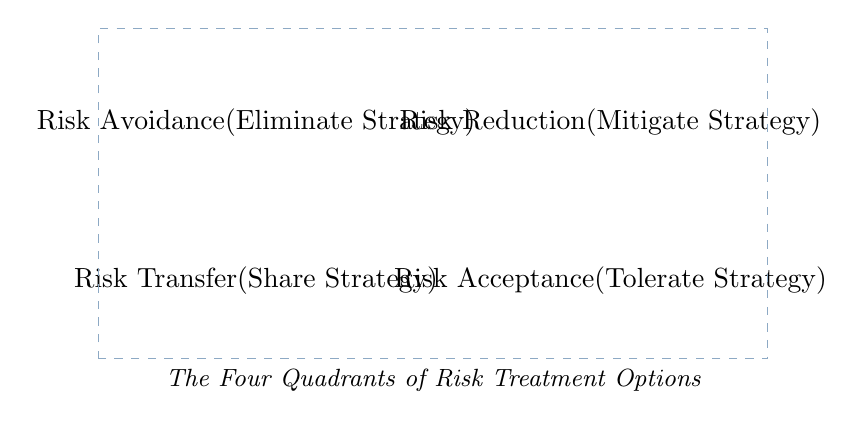
\begin{tikzpicture}[
    node/.style={rectangle, draw=NavyBlue, fill=LightBlue!40, text width=3.2cm, text centered, font=\bfseries\small, minimum height=1.2cm, rounded corners, line width=1pt},
    arrow/.style={thick, ->, >=stealth, draw=DarkBlue, line width=1.2pt}
]
\node (avoid) at (0,2) {Risk Avoidance\\(Eliminate Strategy)};
\node (reduce) at (4.5,2) {Risk Reduction\\(Mitigate Strategy)};
\node (transfer) at (0,0) {Risk Transfer\\(Share Strategy)};
\node (accept) at (4.5,0) {Risk Acceptance\\(Tolerate Strategy)};

\draw[dashed, draw=SlateGray] (-2,-1) rectangle (6.5,3.2);
\node[below] at (2.25,-1) {\small\itshape The Four Quadrants of Risk Treatment Options};
\end{tikzpicture}
\caption{Visual Topology of Risk Management Methodologies}
\label{fig:risk_treatment}
\end{figure}

Let us examine each strategy with precise industry alignment:

\subsubsection{1. Risk Avoidance (Elimination)}
\begin{itemize}[leftmargin=*]
    \item \textbf{Definition:} Modifying corporate operations, system designs, or structural directions entirely to completely strip out the threat variable. This sets the risk score to zero.
    \item \textbf{Corporate Example:} A regional commercial bank wants to deploy a new feature allowing users to upload custom profile pictures. The security audit reveals that malicious actors could embed web shells or steganographic malware within images, risking backend system takeover. The bank decides to \textbf{completely cancel the profile image upload feature}. By avoiding the feature, they avoid the risk entirely.
\end{itemize}

\subsubsection{2. Risk Reduction / Mitigation (Control Application)}
\begin{itemize}[leftmargin=*]
    \item \textbf{Definition:} The process of applying technical, physical, or administrative defensive controls to actively lower either the statistical likelihood of exploitation or the severity of the damage.
    \item \textbf{Corporate Example:} A hospital infrastructure relies on legacy Windows XP terminals to run critical MRI software. This operating system contains massive vulnerabilities. To reduce risk, the IT team disconnects the machines completely from the internet, puts them behind an isolated virtual firewall (VLAN), and mandates physical access keys. The vulnerability remains, but the likelihood of remote cyber exploitation drops dramatically.
\end{itemize}

\subsubsection{3. Risk Transfer / Sharing (Outsourcing or Insurance)}
\begin{itemize}[leftmargin=*]
    \item \textbf{Definition:} Shifting the operational execution or fiscal burden of a risk event to a third-party entity, such as an insurance carrier or a specialized external service provider.
    \item \textbf{Corporate Example:} An e-commerce enterprise handles millions of dollars in customer credit card transactions. Instead of coding and maintaining a highly vulnerable internal processing server (which requires expensive PCI-DSS audits), the company completely outsources its transaction pipeline to \textbf{Stripe/PayPal}. The risk of payment credential theft is transferred onto the specialized processor. Additionally, they purchase a \$5 Million cyber insurance policy to cover legal fees in case of a perimeter breach.
\end{itemize}

\subsubsection{4. Risk Acceptance (Retention)}
\begin{itemize}[leftmargin=*]
    \item \textbf{Definition:} The deliberate management choice to absorb the potential consequences of a specific risk without implementing any active defenses, because the cost of implementing a safeguard far exceeds the maximum loss value of the asset.
    \item \textbf{Corporate Example:} A small marketing firm operates an on-premise server room. A risk assessment identifies that an extremely rare earthquake could destroy the building's physical structure. Buying a highly resilient earthquake-proof underground data bunker would cost \$200,000, while the company's annual profit is only \$50,000. Executive management formally signs a document declaring they \textbf{accept the risk}. They will live with it.
\end{itemize}

\subsection{Step 4: Implement Methods}
This step represents the tactical deployment phase. Management has made its logical decision; now the cyber security engineering and operations teams must build and configure the safeguards.

\begin{definitionbox}{Step 4: Implementation (Exam Definition)}
The operational translation of chosen risk management decisions into tangible, configured infrastructure safeguards categorized under administrative directives, physical barriers, and logical software restrictions.
\end{definitionbox}

\subsubsection{The Three Classic Security Controls Categories}
Students must master the structural classification of defenses:
\begin{enumerate}[leftmargin=*]
    \item \textbf{Technical (Logical) Controls:} Hardened protections implemented via software, hardware, or cryptography. Examples: Deploying Cisco Firewalls, generating AES-256 bit encryption pipelines, activating Multi-Factor Authentication (MFA) protocols, and configuring Intrusion Prevention Systems (IPS).
    \item \textbf{Administrative (Managerial) Controls:} High-level governing procedures driven by human text and organizational constraints. Examples: Mandatory cybersecurity awareness bootcamps for new employees, conducting thorough background verification checks during recruitment, and designing a structured Incident Response Plan (IRP).
    \item \textbf{Physical Controls:} Tangible architectural constraints that shield physical spaces and compute hardware from human hands. Examples: Deploying biometric iris scanners on data center doors, hiring armed campus guards, installing closed-circuit TV (CCTV) cameras, and utilizing automatic gas-based fire suppression systems (FM200).
\end{enumerate}

\subsection{Step 5: Manage and Evaluate}
Cybersecurity is never a static target. The digital landscape shifts constantly. A risk profile that is completely secure on Monday could become fully compromised by Friday due to the discovery of a new Zero-Day exploit code. Step 5 forms the continuous lifecycle oversight loop.

\begin{definitionbox}{Step 5: Manage and Evaluate (Exam Definition)}
The permanent, cyclical oversight phase dedicated to continuous real-time monitoring of deployed security safeguards, regular audits of system infrastructure changes, vulnerability re-assessment, and updating controls to address evolving global threat paradigms.
\end{definitionbox}

\subsubsection{Continuous Monitoring \& Updating Controls}
Analysts execute continuous evaluations via the following mechanisms:
\begin{itemize}[label=$\circ$]
    \item \textbf{SIEM Systems:} Aggregating log data from all endpoints to detect anomalies.
    \item \textbf{Penetration Testing:} Simulating controlled real-world cyber attacks against corporate defenses to test if the controls implemented in Step 4 are actually working.
    \item \textbf{Change Management:} Reviewing whenever a company upgrades its servers, ensuring no new weaknesses are introduced.
\end{itemize}

\begin{examplebox}{Step 5 Operational Breakdown}
A multinational financial institution implements an advanced AI-driven fraud detection control. During the Step 5 review cycle one year later, analysts discover that cybercriminals have learned to use adversarial machine learning to bypass the filter. The security team documents this degradation, updates the underlying algorithmic models, and adjusts the corporate policy. This triggers the entire Risk Analysis process over again.
\end{examplebox}

\newpage
% ==========================================
% SYSTEM VISUALIZATIONS & FLOWCHARTS
% ==========================================
\subsection{Complete Systematic Flow Diagram (TikZ)}
Below is the precise, structured process flow diagram mapping the linear execution and the cyclical optimization loop of enterprise Risk Analysis.

\begin{figure}[htbp]
\centering
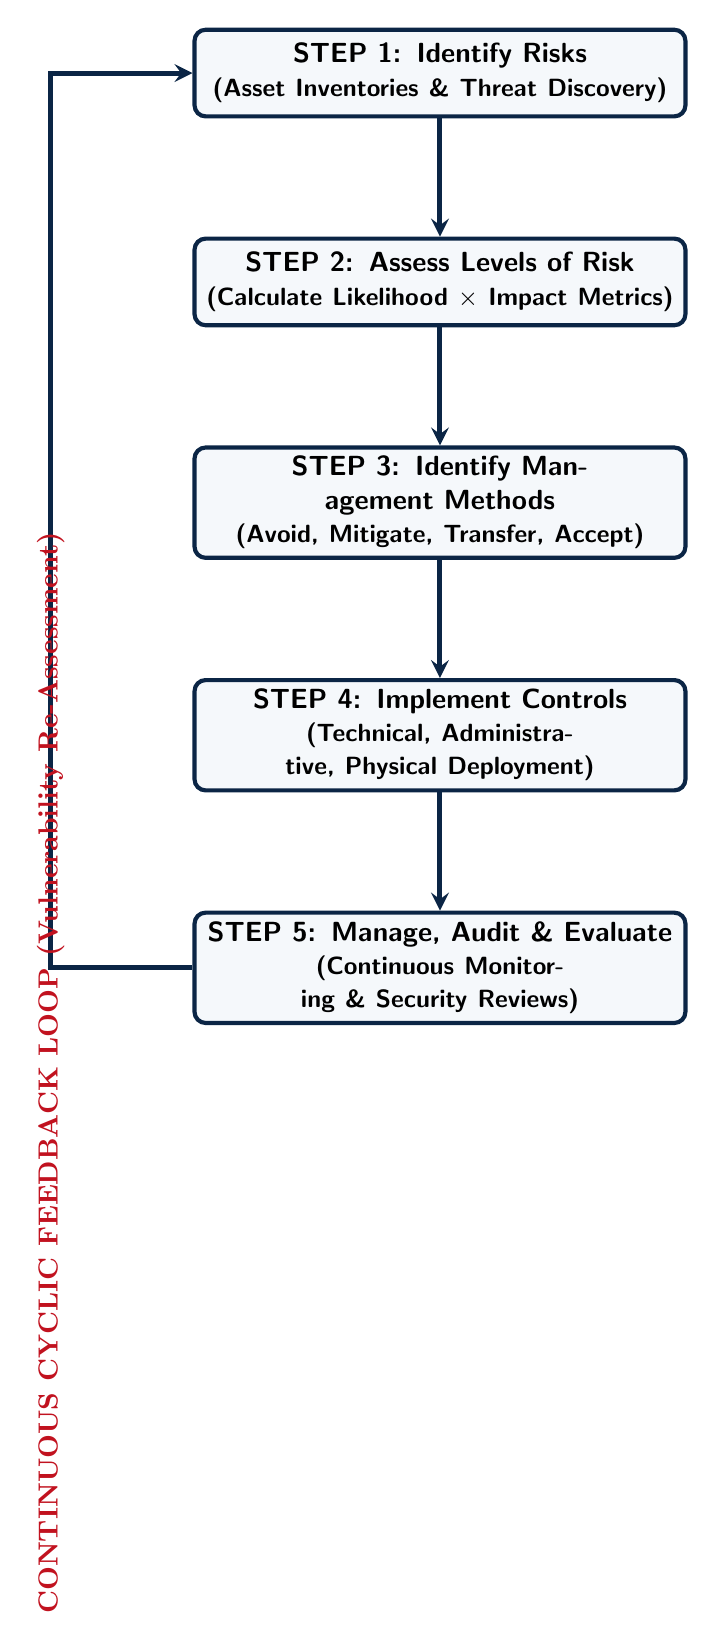
\begin{tikzpicture}[
    node distance=1.5cm,
    block/.style={rectangle, draw=DarkBlue, fill=LightBlue!60, text width=6cm, text centered, rounded corners, minimum height=1.1cm, font=\bfseries\sffamily, line width=1.5pt},
    arrow/.style={thick, ->, >=stealth, draw=DarkBlue, line width=1.8pt}
]
    % Nodes placement
    \node (step1) [block] {STEP 1: Identify Risks\\ \small(Asset Inventories \& Threat Discovery)};
    \node (step2) [block, below=of step1] {STEP 2: Assess Levels of Risk\\ \small(Calculate Likelihood $\times$ Impact Metrics)};
    \node (step3) [block, below=of step2] {STEP 3: Identify Management Methods\\ \small(Avoid, Mitigate, Transfer, Accept)};
    \node (step4) [block, below=of step3] {STEP 4: Implement Controls\\ \small(Technical, Administrative, Physical Deployment)};
    \node (step5) [block, below=of step4] {STEP 5: Manage, Audit \& Evaluate\\ \small(Continuous Monitoring \& Security Reviews)};

    % Linear Arrows
    \draw [arrow] (step1) -- (step2);
    \draw [arrow] (step2) -- (step3);
    \draw [arrow] (step3) -- (step4);
    \draw [arrow] (step4) -- (step5);
    
    % The Eternal Loop Back Arrow
    \draw [arrow] (step5.west) -- ++(-1.8cm,0) |- (step1.west) 
        node[pos=0.25, left, rotate=90, font=\bfseries\color{WarningRed}] {CONTINUOUS CYCLIC FEEDBACK LOOP (Vulnerability Re-Assessment)};

\end{tikzpicture}
\caption{The Structural End-to-End Enterprise Risk Analysis Pipeline}
\label{fig:full_flow_chart}
\end{figure}

\subsection{The Risk Analysis Cycle Topology}
To reinforce the continuous feedback nature of governance, Figure~\ref{fig:circle_topology} shows the conceptual cyclic topology map detailing how security components feed directly into one another.

\begin{figure}[htbp]
\centering
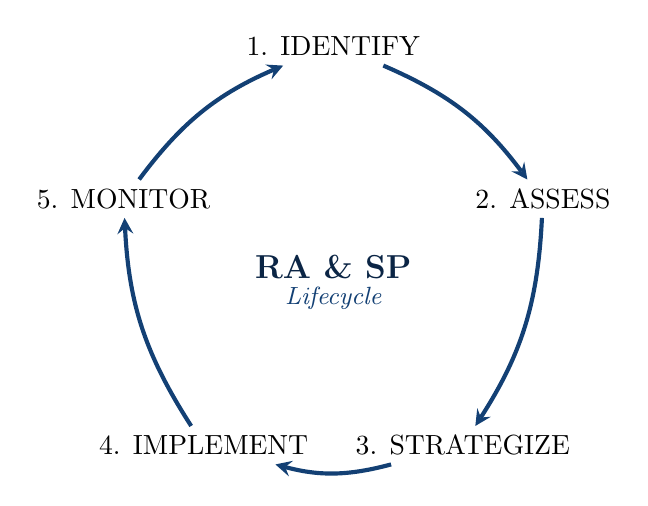
\begin{tikzpicture}[
    node/.style={circle, draw=NavyBlue, fill=LightBlue!30, text width=2cm, text centered, font=\bfseries\sffamily\small, minimum size=2.3cm, line width=1.2pt},
    arrow/.style={thick, ->, >=stealth, draw=NavyBlue, line width=1.5pt}
]
    \node (ident) at (90:2.8cm) {1. IDENTIFY};
    \node (assess) at (18:2.8cm) {2. ASSESS};
    \node (treat) at (306:2.8cm) {3. STRATEGIZE};
    \node (impl) at (234:2.8cm) {4. IMPLEMENT};
    \node (monitor) at (162:2.8cm) {5. MONITOR};

    \draw [arrow] (ident) to[bend left=15] (assess);
    \draw [arrow] (assess) to[bend left=15] (treat);
    \draw [arrow] (treat) to[bend left=15] (impl);
    \draw [arrow] (impl) to[bend left=15] (monitor);
    \draw [arrow] (monitor) to[bend left=15] (ident);
    
    \node at (0,0) [font=\bfseries\color{DarkBlue}\large] {RA \& SP};
    \node at (0,-0.4) [font=\small\itshape\color{NavyBlue}] {Lifecycle};
\end{tikzpicture}
\caption{The Eternal Circular Architecture of Cybersecurity Risk Governance}
\label{fig:circle_topology}
\end{figure}

\newpage

% ==========================================
% SECTION: CASE STUDY
% ==========================================
\subsection{Practical University Case Study}
\textbf{Scenario:} \textit{Hamdard University Islamabad Campus (HUIC)} is deploying a centralized database system called "HUIC Cloud Student Records" to host all grades, exams, transcripts, and financial clearance data. If this system is compromised, academic integrity collapses, and operations freeze. Let us apply the 5 Steps of Risk Analysis.

\begin{enumerate}[leftmargin=*]
    \item \textbf{Step 1: Identify Risks:}
    \begin{itemize}
        \item \textit{Asset Identification:} The primary asset is the SQL Student Records database containing exam grading matrices.
        \item \textit{Threat Discovery:} Tech-savvy students seeking to maliciously inflate their final GPAs prior to graduation.
        \item \textit{Vulnerability Assessment:} The web portal interface lacks input filtering, making it highly susceptible to standard \textbf{SQL Injection (SQLi)} exploit payloads.
    \end{itemize}
    \item \textbf{Step 2: Assess Event to Determine Levels of Risk:}
    \begin{itemize}
        \item \textit{Likelihood Assessment:} Highly Motivated threat actors with available scripts online ($\text{Likelihood Score} = 4/\text{Likely}$).
        \item \textit{Impact Assessment:} Arbitrary database rewriting completely invalidates the university degree authority, leading to full operational loss ($\text{Impact Score} = 5/\text{Catastrophic}$).
        \item \textit{Final Valuation:} Matrix cross-reference sets this as a \textbf{Critical Risk Level}.
    \end{itemize}
    \item \textbf{Step 3: Identify Methods to Manage Risk:}
    The academic board analyzes cost/feasibility paths:
    \begin{itemize}
        \item \textit{Avoidance Option:} Cancel the cloud database entirely and return to physical handwritten paper ledger ledgers locked in metal safes. (Rejected due to high efficiency costs).
        \item \textit{Transfer Option:} Buy cyber insurance. (Insufficient to restore damaged reputation).
        \item \textit{Mitigation Selection:} Implement strict multi-tiered engineering security controls to bring the risk level down to an acceptable baseline.
    \end{itemize}
    \item \textbf{Step 4: Implement Methods:}
    The university engineering unit actively deploys:
    \begin{itemize}
        \item \textit{Technical Controls:} Hardening the database web front-end with parameterized queries and strict input validation rules; installing a Web Application Firewall (WAF).
        \item \textit{Administrative Controls:} Enforcing a strict \textit{Least Privilege Policy} whereby only authorized professors can alter fields under a dual-authorization check loop.
        \item \textit{Physical Controls:} Locking the database servers in an air-conditioned datacenter vault protected by smartcard biometric authentication.
    \end{itemize}
    \item \textbf{Step 5: Manage and Evaluate:}
    Every six months, HUIC hires an independent external penetration testing group to attempt to exploit the student web portal. The IT division reviews firewall drop logs weekly, ensuring that new SQL injection bypass methodologies discovered globally are updated in the WAF filter signature files.
\end{enumerate}

\subsection{Core Organizational Advantages}
\begin{itemize}[leftmargin=*]
    \item \textbf{Proactive vs. Reactive Posture:} Prevents catastrophic security data breaches from occurring rather than dealing with the massive financial cleanup cost after a hack.
    \item \textbf{Informed Budgeting:} Provides empirical data tables to senior management, proving why specific firewall infrastructure buys are needed.
    \item \textbf{Enhanced Institutional Trust:} Clients, patients, and student bodies confidently conduct transactions knowing their private data matches hardened standards.
\end{itemize}

\newpage

% ==========================================
% OFFICIAL UNIVERSITY EXAMINATION BANK
% ==========================================
\section{Official University Examination Bank}

This section is custom-tailored to prepare students for the rigorous formatting of formal university midterms, finals, and viva examinations.

\subsection{Core Exam Tips}
\begin{examtipbox}
When writing answers for formal scoring, keep these parameters in mind:
\begin{enumerate}[leftmargin=*]
    \item \textbf{Do Not Confuse Threat and Risk:} A threat is the agent (e.g., Ransomware). A risk is the calculation of an event happening ($\text{Likelihood} \times \text{Impact}$). Writing "Ransomware is a risk" loses marks. You must write "The risk of ransomware exploiting unpatched network ports to lock data, resulting in operations downtime."
    \item \textbf{Always State the Framework Formula:} Whenever defining risk, explicitly write out $\text{Risk} = \text{Likelihood} \times \text{Impact}$ to claim absolute definition points automatically.
    \item \textbf{Classification Clarity:} In questions asking for security controls, cleanly split your paragraphs into Technical, Administrative, and Physical subheadings. Bulleted blocks receive higher evaluations than long unstructured text paragraphs.
\end{enumerate}
\end{examtipbox}

\subsection{Common Student Mistakes to Avoid}
\begin{warningbox}
Avoid these common conceptual pitfalls in your exam sheets:
\begin{itemize}[leftmargin=*]
    \item \textbf{The 100\% Security Myth:} Claiming that applying risk reduction makes a system "100\% completely secure or bulletproof." This is technically impossible. Residual risk always remains.
    \item \textbf{Misunderstanding Avoidance:} Confusing Risk Avoidance with Risk Mitigation. Avoidance means \textbf{completely dropping the asset or business process}. If you still run the database but put three firewalls in front of it, you are \textbf{Mitigating}, not avoiding.
    \item \textbf{Passive Registers:} Believing that a Risk Register is a one-time project. It is a living document that must be continuously evaluated.
\end{itemize}
\end{warningbox}

% ------------------------------------------
% MCQS SECTION
% ------------------------------------------
\subsection{Multiple Choice Questions (MCQs)}

1. An inherent structural flaw, loophole, or weakness within an operating system or organization is formally termed as a/an: \\
A) Threat \hfill B) Vulnerability \\
C) Risk \hfill D) Impact \\
\textbf{Answer: B} \\
\textit{Explanation:} Vulnerabilities represent internal weaknesses. Threats are external destructive events that seek to exploit these weaknesses.

2. A high-level cybersecurity governance directive signed and issued by senior enterprise executives to define behavioral boundaries is a/an: \\
A) Risk Register \hfill B) Security Control \\
C) Security Policy \hfill D) Asset Inventory \\
\textbf{Answer: C} \\
\textit{Explanation:} Security policies represent administrative governance mandates set by top management.

3. Which specific risk response strategy is being executed when an e-commerce platform decides to completely delete its digital payment database and outsource all credit card transactions to PayPal? \\
A) Risk Mitigation \hfill B) Risk Acceptance \\
C) Risk Avoidance \hfill D) Risk Transfer \\
\textbf{Answer: D} \\
\textit{Explanation:} Shifting the operational and legal burden of data processing to a third party constitutes Risk Transfer.

4. A security analyst maps a highly complex threat event that has an automated frequency score of 5 (Almost Certain) but affects public marketing documentation with an impact score of 1 (Insignificant). The matrix risk ranking is: \\
A) Critical \hfill B) High \\
C) Medium \hfill D) Low \\
\textbf{Answer: C / Low-Medium depending on matrix} \\
\textit{Explanation:} Based on standard mathematical models, $5 \times 1 = 5$, which positions the hazard toward a lower corporate priority due to non-existent structural damage.

5. Biometric readers, automatic gas fire suppression modules, and perimeter steel fences are explicitly classified under which control category? \\
A) Technical Controls \hfill B) Administrative Controls \\
C) Physical Controls \hfill D) Logical Controls \\
\textbf{Answer: C} \\
\textit{Explanation:} Anything tangible that physically blocks human contact with computational hardware falls under physical design constraints.

6. The mathematical expression utilized to model basic semi-quantitative risk values is: \\
A) $\text{Risk} = \text{Threat} + \text{Vulnerability}$ \hfill B) $\text{Risk} = \text{Likelihood} \times \text{Impact}$ \\
C) $\text{Risk} = \text{Asset Value} / \text{Countermeasure}$ \hfill D) $\text{Risk} = \text{Impact} - \text{Likelihood}$ \\
\textbf{Answer: B} \\
\textit{Explanation:} Industrial frameworks multiply probability by loss value to output core metric vectors.

7. Which step of the Risk Analysis lifecycle framework is specifically focused on the discovery and compiling of all systems, hardware components, and corporate assets? \\
A) Step 4: Implementation \hfill B) Step 2: Assessment \\
C) Step 5: Evaluation \hfill D) Step 1: Identification \\
\textbf{Answer: D} \\
\textit{Explanation:} Identification builds the initial repository foundation by discovering assets, threats, and current exploits.

8. If a business enterprise formally decides that the cost of mitigating a low-level risk is higher than the maximum possible loss of the asset itself, and chooses to do nothing, they are performing: \\
A) Risk Avoidance \hfill B) Risk Acceptance \\
C) Risk Sharing \hfill D) Risk Transmutation \\
\textbf{Answer: B} \\
\textit{Explanation:} Risk acceptance means acknowledging the vulnerability but choosing to live with it due to rational cost-benefit analysis.

9. What is the core relationship between Risk Analysis and Security Policies? \\
A) They are identical concepts. \hfill B) Security Policies are written first to guide Risk Analysis. \\
C) Risk Analysis provides the empirical diagnoses that drives specific Security Policy rules. \hfill D) Risk Analysis completely replaces the need for policies. \\
\textbf{Answer: C} \\
\textit{Explanation:} Analysis uncovers system realities; policies enforce the required operational constraints to manage those realities.

10. The continuous process of running vulnerability scans, analyzing network traffic logs via SIEMs, and updating controls over time is detailed under which step? \\
A) Step 2 \hfill B) Step 5 \\
C) Step 3 \hfill D) Step 1 \\
\textbf{Answer: B} \\
\textit{Explanation:} Step 5 is the continuous evaluation, maintenance, and audit phase of the lifecycle loop.

% ------------------------------------------
% VIVA QUESTIONS
% ------------------------------------------
\subsection{Viva Voce Oral Examination Questions}
\begin{enumerate}[leftmargin=*]
    \item \textbf{Question:} \textit{"Explain the difference between a Vulnerability and a Threat to an undergraduate panel."} \\
    \textbf{Answer:} A vulnerability is an internal weakness or flaw present in our system design or codebase (e.g., an unpatched software bug). A threat is an external or internal entity or event that has the potential to exploit that weakness maliciously (e.g., a professional hacker running an automated exploit tool).
    \item \textbf{Question:} \textit{"Can an organization ever achieve Zero Risk? Why or why not?"} \\
    \textbf{Answer:} No, zero risk is a theoretical myth. The moment a system is turned on or connected to a network, risk is introduced. New vulnerabilities are discovered daily, and humans make mistakes. We can only mitigate risk down to an acceptable level known as Residual Risk.
    \item \textbf{Question:} \textit{"What is a Risk Register, and when do you create it?"} \\
    \textbf{Answer:} A Risk Register is a dynamic living database spreadsheet created during Step 1 (Identification) of the Risk Analysis framework. It acts as an absolute master inventory cataloging every single identified asset, its vulnerabilities, mapped threats, and its ultimate risk score.
    \item \textbf{Question:} \textit{"Give me an example of a technical control versus an administrative control in a bank."} \\
    \textbf{Answer:} A technical control would be deploying an AES-256 bit encryption engine over the bank's account database. An administrative control would be writing a mandatory corporate policy document stating that employees will be immediately fired if they share their account passwords.
    \item \textbf{Question:} \textit{"What is the core difference between Risk Mitigation and Risk Avoidance?"} \\
    \textbf{Answer:} Risk Mitigation means keeping the business asset or process operational but applying security controls to lower the threat score. Risk Avoidance means completely removing the asset or canceling the project entirely to eliminate the risk vector altogether.
    \item \textbf{Question:} \textit{"Why is Step 5 (Manage and Evaluate) drawn as a loop back to Step 1?"} \\
    \textbf{Answer:} Because the security environment changes constantly. A system that is safe today might see new vulnerabilities released tomorrow. The continuous loop forces the organization to constantly re-identify and re-assess their system defenses.
    \item \textbf{Question:} \textit{"What do we mean by business asset impact?"} \\
    \textbf{Answer:} Impact is the total severity of consequences an organization suffers if a threat successfully compromises an asset. It is measured in financial losses, hours of system downtime, regulatory legal lawsuits, or permanent brand reputational ruin.
    \item \textbf{Question:} \textit{"What occurs if an organization writes a Security Policy without running a Risk Analysis first?"} \\
    \textbf{Answer:} The policy becomes blind, generic guesswork. It will mandate rules that protect against irrelevant threats while leaving actual critical weaknesses completely undefended, frustrating workers and wasting money.
    \item \textbf{Question:} \textit{"What is the role of a $5 \times 5$ Risk Matrix?"} \\
    \textbf{Answer:} It is a visual prioritization tool that plots likelihood frequency on one axis against consequence impact on the other. It helps executives instantly categorize risks into low, medium, high, or critical bands so they know where to spend money first.
    \item \textit{"Define a countermeasure in your own words."} \\
    \textbf{Answer:} A countermeasure is any action, process, software tool, or physical device deployed as a defensive wall to stop a threat from reaching a vulnerability.
\end{enumerate}

% ------------------------------------------
% SHORT QUESTIONS
% ------------------------------------------
\subsection{Short Answer Written Questions (2 Marks Each)}

\subsubsection{Q1: Define the term 'Residual Risk' in professional frameworks.}
\textbf{Model Answer:} Residual Risk is the leftover baseline risk that remains within an information infrastructure even after all planned technical, administrative, and physical security controls have been correctly implemented. It represents the permanent risk an organization formally agrees to live with.

\subsubsection{Q2: State the primary objectives of Step 1 (Risk Identification).}
\textbf{Model Answer:} The dual objectives are: first, to build a complete, non-blind inventory map of all tangible and intangible organizational assets; second, to systematically uncover and catalog corresponding internal system vulnerabilities and active external threat agents into a formal corporate Risk Register.

\subsubsection{Q3: Differentiate between Quantitative and Qualitative Risk Analysis.}
\textbf{Model Answer:} Quantitative Analysis assigns concrete monetary and numerical values to assets and risks (e.g., a risk costing exactly \$45,000 in cash). Qualitative Analysis utilizes descriptive, subjective rankings based on judgment and experience (e.g., grading a threat as "High Risk" or "Low Risk" on a color-coded matrix).

\subsubsection{Q4: What specific questions must an analyst answer during Step 2 (Risk Assessment)?}
\textbf{Model Answer:} The analyst must explicitly resolve two questions:
1. \textit{"What is the exact statistical likelihood or frequency of this specific vulnerability being successfully exploited by the threat agent?"}
2. \textit{"What is the exact scale of operational, financial, or legal impact loss if the breach succeeds?"}

\subsubsection{Q5: Provide two distinct real-world examples of a Physical Control inside a corporate hospital environment.}
\textbf{Model Answer:}
1. Installing electronic biometric fingerprint access locks on the data room entry doors where local electronic medical record servers are physically housed.
2. Mounting high-definition CCTV security cameras inside server corridors to establish permanent visual tracking logs of all physical human movement.

% ------------------------------------------
% MEDIUM QUESTIONS
% ------------------------------------------
\subsection{Medium Answer Analytical Questions (5 Marks Each)}

\subsubsection{Q1: Explain the structural mechanics of the Four Risk Treatment Strategies, providing a distinct corporate example for each.}
\textbf{Model Answer:} The four strategies allow an organization to properly handle assessed risks:
\begin{itemize}[leftmargin=*]
    \item \textbf{Avoidance:} Complete termination of the high-risk activity or system. \textit{Example:} A company completely cancels the deployment of a new mobile app because the software is too vulnerable to remote API data extraction.
    \item \textbf{Mitigation:} Applying active controls to lower likelihood or impact. \textit{Example:} Enforcing corporate-wide Multi-Factor Authentication (MFA) to stop credential-stuffing attacks.
    \item \textbf{Transfer:} Shifting the financial or operational burden to a third party. \textit{Example:} Outsourcing processing infrastructure to specialized cloud vendors or purchasing comprehensive corporate cyber insurance policies.
    \item \textbf{Acceptance:} Consciously choosing to tolerate the risk without adding defenses due to positive cost-benefit justification. \textit{Example:} Living with the risk of a minor public website typo because the correction cost outweighs any imaginary reputational damage.
\end{itemize}

\subsubsection{Q2: Analyze the role of Step 5 (Manage and Evaluate) in maintaining enterprise infrastructure resilience. Why is it a fatal mistake to treat Risk Analysis as a one-time standalone project?}
\textbf{Model Answer:} Step 5 represents the lifecycle continuous governance phase. Treat risk evaluation as a single static event creates immediate security blindspots. Global cyber landscapes are dynamically evolving; software vendors release new patches, hackers write new automated exploits, and organizations modify internal networks. 

If a company runs an analysis only once, their controls will rapidly degrade against newly discovered vulnerabilities. Step 5 enforces continuous vulnerability re-assessments, network security baseline penetration testing, and policy modifications to ensure corporate defenses adapt to real-world threats.

% ------------------------------------------
% LONG QUESTIONS
% ------------------------------------------
\subsection{Long Essay/Comprehensive Questions (10 Marks Each)}

\subsubsection{Q1: Provide an exhaustive breakdown of the entire Five-Step Risk Analysis Framework. For every individual stage, define its technical purpose, operational components, explicit deliverables, and apply the concept sequentially to a global commercial bank deploying an online customer portal application.}
\textbf{Model Answer:}
\textbf{Introduction:} The five-step framework provides a structured methodology to translate chaos into systematic risk management. Let us map each phase with its purpose, actions, and deliverables applied to a commercial banking online portal application.

\textbf{Step 1: Identify Risks}
\begin{itemize}
    \item \textit{Technical Purpose:} Establish an absolute directory baseline of what needs defense and what threats exist.
    \item \textit{Operational Actions:} The bank logs its assets (customer web portal source code, database servers storing account balances). They map threats (organized cybercrime rings, phishing syndicates) and vulnerabilities (web app input field lacks sanitization, exposing it to Cross-Site Scripting or SQL injection).
    \item \textit{Deliverable:} A formal bank Risk Register cataloging these variables.
\end{itemize}

\textbf{Step 2: Assess Event to Determine Levels of Risk}
\begin{itemize}
    \item \textit{Technical Purpose:} Establish prioritized risk scores to guide corporate spending.
    \item \textit{Operational Actions:} The banking analysts review historical attack data. SQL injection attempts are constant globally ($\text{Likelihood} = 5/\text{Almost Certain}$). The compromise of the core account database allows arbitrary balance manipulation ($\text{Impact} = 5/\text{Catastrophic}$). The matrix calculation fields a critical score ($5 \times 5 = 25$).
    \item \textit{Deliverable:} A prioritized Risk Heat Map.
\end{itemize}

\textbf{Step 3: Identify Methods to Manage Risk}
\begin{itemize}
    \item \textit{Technical Purpose:} Choose the most logical strategy (Avoid, Mitigate, Transfer, Accept).
    \item \textit{Operational Actions:} Executive management realizes they cannot avoid the risk (canceling online banking would destroy their market share) and cannot simply accept it (bankruptcy). They choose a hybrid approach: \textbf{Transferring} parts of the fiscal risk via cyber insurance, and heavily \textbf{Mitigating} the software infrastructure via engineering controls.
    \item \textit{Deliverable:} Formally signed Risk Treatment Plan directives.
\end{itemize}

\textbf{Step 4: Implement Methods}
\begin{itemize}
    \item \textit{Technical Purpose:} Deploy actual safeguards to harden the architecture.
    \item \textit{Operational Actions:} The bank's engineers build a series of defensive walls:
    \begin{enumerate}
        \item \textit{Technical Controls:} Hardening the application codebase with parameterized queries; deploying a redundant Web Application Firewall (WAF); forcing mandatory multi-factor authentication (MFA).
        \item \textit{Administrative Controls:} Creating strict background check policies for database admins; enforcing separation of duties.
        \item \textit{Physical Controls:} Putting server mainframes into biometric-locked data vault rooms monitored by 24/7 security staff.
    \end{enumerate}
    \item \textit{Deliverable:} Configured production architecture with active security validation logs.
\end{itemize}

\textbf{Step 5: Manage and Evaluate}
\begin{itemize}
    \item \textit{Technical Purpose:} Maintain the security posture against real-world degradation.
    \item \textit{Operational Actions:} The bank continuously aggregates logs via SIEM software tools. They hire certified external ethical hackers quarterly to perform rigorous penetration tests against the online portal, looking for newly discovered zero-day exploits. If structural flaws emerge, the cycle restarts immediately at Step 1 to keep defenses updated.
    \item \textit{Deliverable:} Audit compliance logs, vulnerability assessment reports, and patch management schedules.
\end{itemize}

% ------------------------------------------
% SCENARIO-BASED QUESTIONS
% ------------------------------------------
\subsection{Scenario-Based Engineering Problems}

\subsubsection{Scenario A: The Vulnerable Medical Records API}
\textbf{Problem Scenario Description:} You are hired as the Lead Cyber Security Governance Consultant for \textit{Metro Health Systems}. The hospital has deployed an internet-exposed Application Programming Interface (API) to allow mobile applications to quickly pull patient blood reports. 

An internal digital forensics audit discovers that the API does not validate session tokens, meaning anyone with basic web knowledge can modify the URL parameters to view any patient's full medical history. Executive board members want to ignore the flaw because fixing the source code will cost \$15,000 in software developer hours, and they believe "hackers do not care about blood reports."

\textbf{Your Task as an Analyst:} Write a formal, structured response using the terminology learned in Lecture 1 (Asset, Threat, Vulnerability, Risk, Impact, Security Policy) to convince the board to change their mind. Map out the flaw using the 5 Steps of Risk Analysis to show them the real danger.

\textbf{Solution Analysis \& Architectural Answer:}
To convince the executive board, we must translate this technical flaw into a clear business impact using formal risk parameters:
\begin{itemize}[leftmargin=*]
    \item \textbf{Asset Mapping:} The asset is not just a "blood report." It is the hospital's central confidential patient database, which contains Protected Health Information (PHI). This data is highly valuable on the dark web and carries strict legal protections.
    \item \textbf{Vulnerability Identification:} The complete lack of API session token validation represents a critical system vulnerability.
    \item \textbf{Threat Matrix:} The threat agent includes malicious external attackers, identity thieves, and malicious actors looking for ransom opportunities.
    \item \textbf{Risk Calculation:} The risk is that an external actor easily runs an automated script to scrape the entire database, leading to a massive data breach.
\end{itemize}

Let us apply the \textbf{Five-Step Risk Framework} to illustrate the severity:
\begin{enumerate}
    \item \textbf{Step 1 (Identify):} We have documented a critical asset (PHI) exposed to a highly motivated threat via an elementary software vulnerability (lack of token checks).
    \item \textbf{Step 2 (Assess):} The likelihood is scored as \textbf{5 (Almost Certain)} because the API is fully exposed to the public internet and requires zero hacking tools to exploit. The business impact is scored as \textbf{5 (Catastrophic)} because leaking patient data triggers massive regulatory fines under healthcare privacy laws (e.g., HIPAA), immediate class-action lawsuits, and permanent damage to the hospital's reputation. $\text{Total Risk Score} = 5 \times 5 = 25$ (\textbf{Critical Enterprise Threat}).
    \item \textbf{Step 3 \& 4 (Strategize \& Implement):} The board's preference to accept the risk is a severe mistake. A \$15,000 mitigation cost is insignificant compared to millions in legal penalties and regulatory fines. The bank must enforce \textbf{Risk Mitigation}. They need to implement a technical control: rewrite the API code to enforce robust OAuth 2.0 token authentication.
    \item \textbf{Step 5 (Evaluate):} Mandate automated weekly API vulnerability scanning to ensure no future updates accidentally remove the token validation rules.
\end{enumerate}
\textbf{Conclusion Directive:} The hospital's current \textit{Information Security Policy} explicitly mandates the protection of patient confidentiality. Ignoring this vulnerability violates corporate policy and exposes the board to direct personal liability for regulatory non-compliance. Mitigation must begin immediately.

\newpage

% ==========================================
% ONE PAGE REVISION SHEET / CHEAT SHEET
% ==========================================
\section{One-Page Exam Revision Cheat Sheet}

This condensed reference matrix is designed for rapid review right before entering the examination room. It condenses all core concepts from Lecture 1 into a high-density keyword summary.

\begin{longtable}{p{3.2cm}<{\bfseries}p{5.5cm}p{6.5cm}}
\caption{High-Density Revision Matrix for Lecture 1} \\
\toprule
\rowcolor{DarkBlue} \color{white}Core Framework Component & \color{white}Essential Concept Definitions & \color{white}Core Exam Keywords for Full Marks \\ \midrule
\end{firsthead}
\toprule
\rowcolor{DarkBlue} \color{white}Core Framework Component & \color{white}Essential Concept Definitions & \color{white}Core Exam Keywords for Full Marks \\ \midrule
\end{head}
\textbf{Risk} & Likelihood multiplied by Impact. & $\text{Risk} = \text{Likelihood} \times \text{Impact}$, Threat exploiting Vulnerability, Loss Magnitude. \\ \addlinespace
\textbf{Risk Analysis} & Systematic diagnostic process identifying and prioritizing system vulnerabilities. & Structured Assessment, Asset Valuation, Risk Register compilation, Cost-Benefit Baseline. \\ \addlinespace
\textbf{Security Policy} & High-level corporate rulebook defining user limits and security boundaries. & Executive Management Directive, Mandatory Compliance, Disciplinary Actions, Governance Framework. \\ \addlinespace
\textbf{Vulnerability} & Internal system flaw, loop-hole, or structural weakness. & Bug, Missing Patch, Weak Password, Lack of training, Inherent flaw. \\ \addlinespace
\textbf{Threat} & External or internal active agent capable of causing asset damage. & Adversary, Attacker, Natural Disaster, Threat Actor, Malicious Intent. \\ \addlinespace
\textbf{Step 1: Identify} & Discovering and cataloging everything inside the ecosystem. & Asset Discovery, Vulnerability Assessment, Threat Mapping, Risk Register creation. \\ \addlinespace
\textbf{Step 2: Assess} & Calculating risk severity scores to prioritize remediation. & Probability Matrix, $5 \times 5$ Grid, Qualitative Scoring, Priority Level (Low/High/Critical). \\ \addlinespace
\textbf{Step 3: Strategize} & Selecting the high-level business path to handle the risk. & Avoidance (Eliminate), Mitigation (Reduce), Transfer (Share), Acceptance (Tolerate). \\ \addlinespace
\textbf{Step 4: Implement} & Deploying tactical safeguards across the infrastructure. & Technical (Firewalls/MFA), Administrative (Policies/IRP), Physical (Locks/Guards). \\ \addlinespace
\textbf{Step 5: Monitor} & Cyclical oversight loop auditing system changes over time. & Continuous Evaluation, SIEM Auditing, Penetration Testing, Cyclic Feedback Loop. \\
\bottomrule
\end{longtable}

\subsection{Lecture Summary}
In this introductory lecture, we transformed the subjective, everyday concept of "risk" into a rigorous mathematical and analytical model: $\text{\bfseries Risk} = \text{\bfseries Likelihood} \times \text{\bfseries Impact}$. 

You learned that proactive \textbf{Risk Analysis} serves as the critical diagnostic assessment that exposes an organization's hidden technical flaws and vulnerabilities, while corporate \textbf{Security Policies} provide the official, mandatory rules and governance frameworks required to deploy and enforce real-world defenses. 

By mastering the standardized \textbf{Five-Step Risk Analysis Framework}—stretching from the initial identification of assets in Step 1 to the continuous, cyclical monitoring and auditing in Step 5—you are now fully equipped to analyze enterprise infrastructures through a strategic lens. This mindset shifts your focus from merely identifying security bugs to actively defending business value. This foundational strategy will guide every architectural module you encounter throughout your BS DFCS degree program.

\end{document}
